%
\chapter{Vzorec poročila o opravljenem delu in o spoznanjih}
\label{ch:Poroc_Vzorec} % Always give a unique label
% use \chaptermark{}
% to alter or adjust the chapter heading in the running head

Primer kako študentje napišejo poročilo.

\section{Usposabljanje girokompasa}	
\label{sec:1}
% Always give a unique label
% and use \ref{<label>} for cross-references
% and \cite{<label>} for bibliographic references
% use \sectionmark{}
% to alter or adjust the section heading in the running head
Študentje: L. Toplikar, A. Bjelanović, A. Lupše, G. Potočnik, L. Lah //Mentor: F. Dimc.

\begin{figure}
	\centering
	% Use the relevant command for your figure-insertion program
	% to insert the figure file.
	% For example, with the option graphics use
	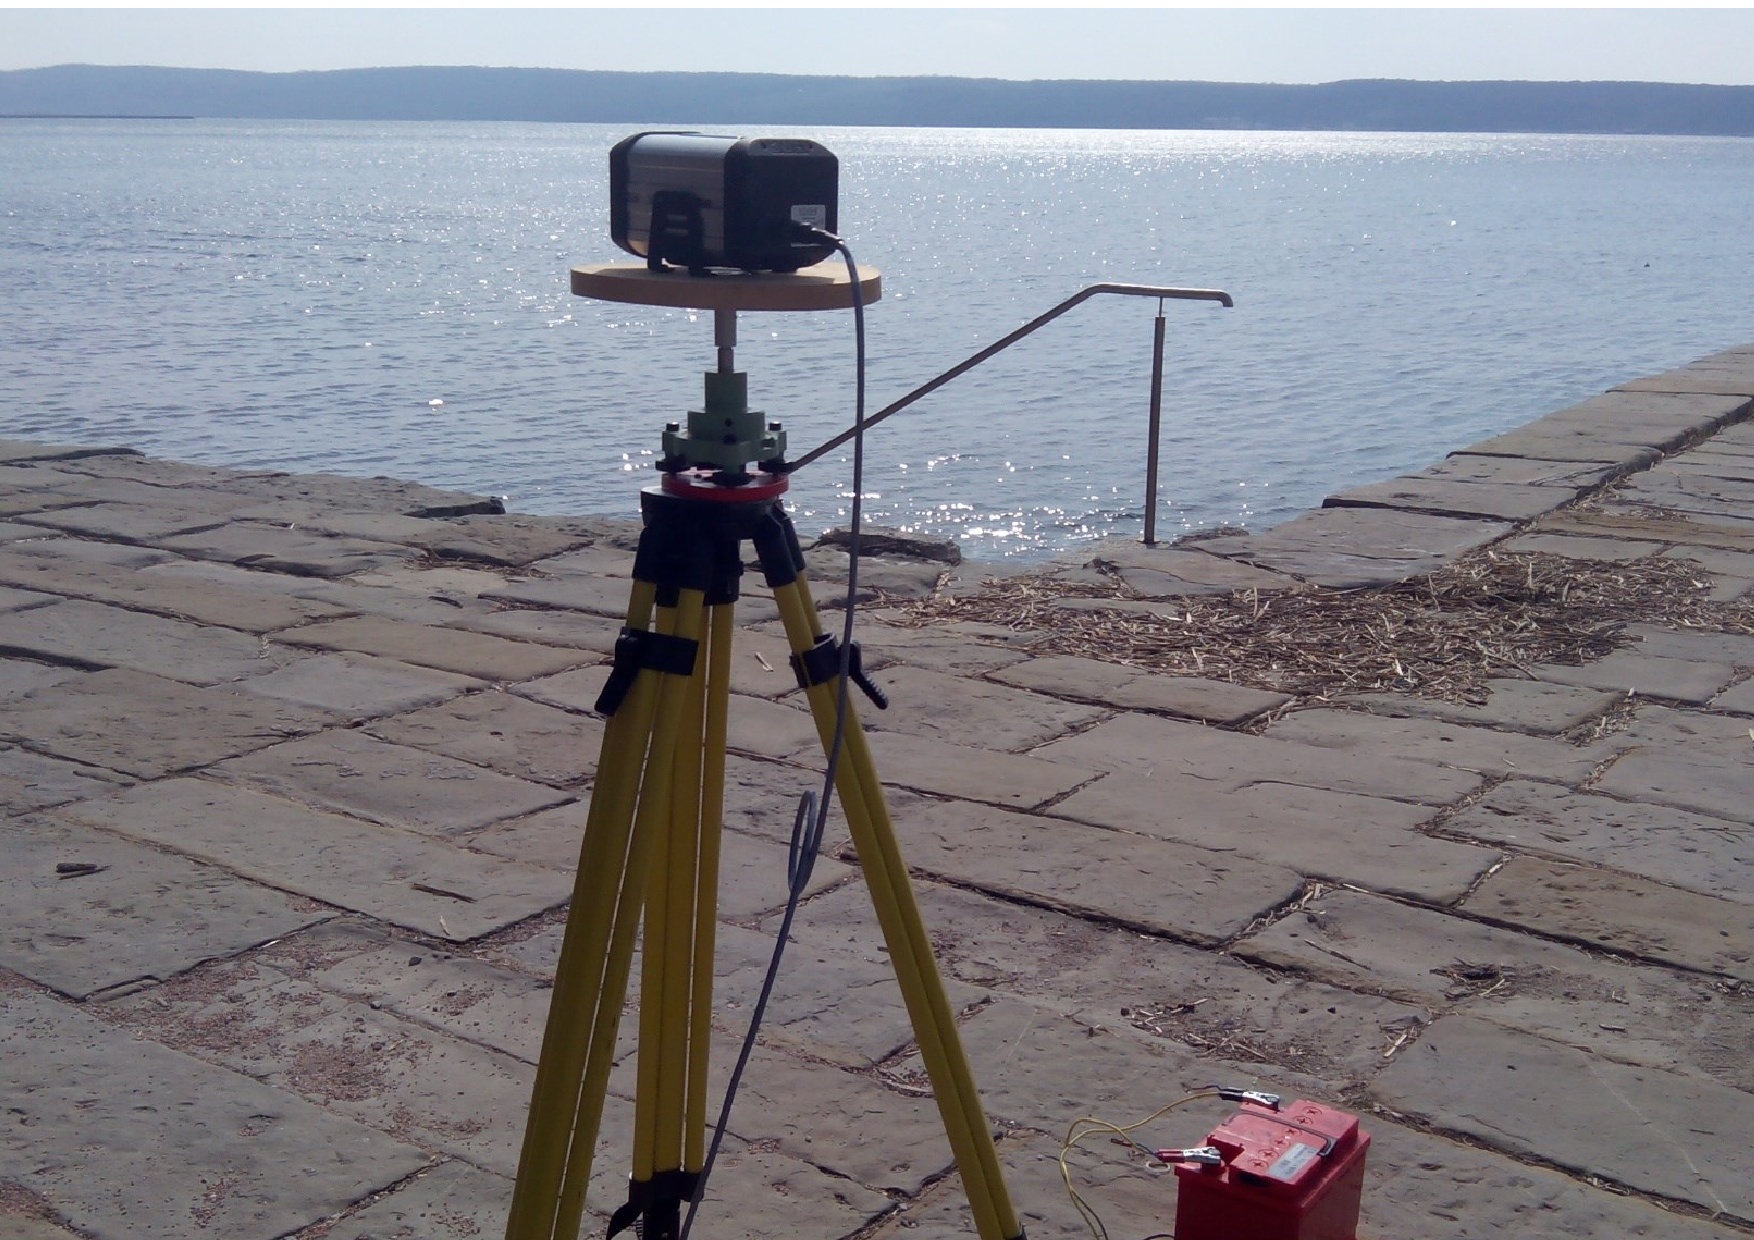
\includegraphics[height=5cm]{Vaje/VzorecPoroc/figs/Gyro_obala.pdf}
	%
	% If not, use
	%\picplace{5cm}{2cm} % Give the correct figure height and width in cm
	%
	\caption{Postavitev kompasa na obali}
	\label{fig:Gyro_obala}       % Give a unique label
\end{figure}

\subsection{Uvod}
%\label{sec:2}
Delo se je začelo z osnovanjem skupin. Ko so bile skupine sestavljene, je profesor vsaki dal pisna navodila. Naša skupina je prejela navodila za usposabljanje girokompasa. Profesor nam je poslal literaturo  \cite{Girokompas_2012}, \cite{Girokompas_2013} ter navodila naprave \cite{Gyro_Man}, kar smo preučili.

Naš del raziskovanja smo začeli tako, da smo najprej naprave preizkusili povezati in usposobiti v laboratoriju s pomočjo profesorja. Ko nam je to uspelo, smo se zmenili za gomon Valentino in poskuse izvedli na morju. Pred odhodom na morje smo še enkrat povezali naprave, da smo preverili ali vse res deluje.

\subsubsection{Naloga}
Naša naloga je bila, da z girokompasom, montiranim na gomon, izmerimo pokrito smer na svetilnika in le-to primerjamo s smerjo izmerjeno na karti. Določiti smo morali tudi reakcijski čas girokompasa.

\subsubsection{Opis naprav}
Naprave, ki smo jih uporabili, so bile:
\begin{itemize}
	\item \textbf{kompas} Girotrack s prikazovalnikom ADCU, 
	\item \textbf{računalnik} s programom Tera Term, 
	\item \textbf{pretvornik} ATEN uc4854 in 
	\item \textbf{akumulator} za napajanje.
\end{itemize}  

\begin{figure}
	\centering
	% Use the relevant command for your figure-insertion program
	% to insert the figure file.
	% For example, with the option graphics use
	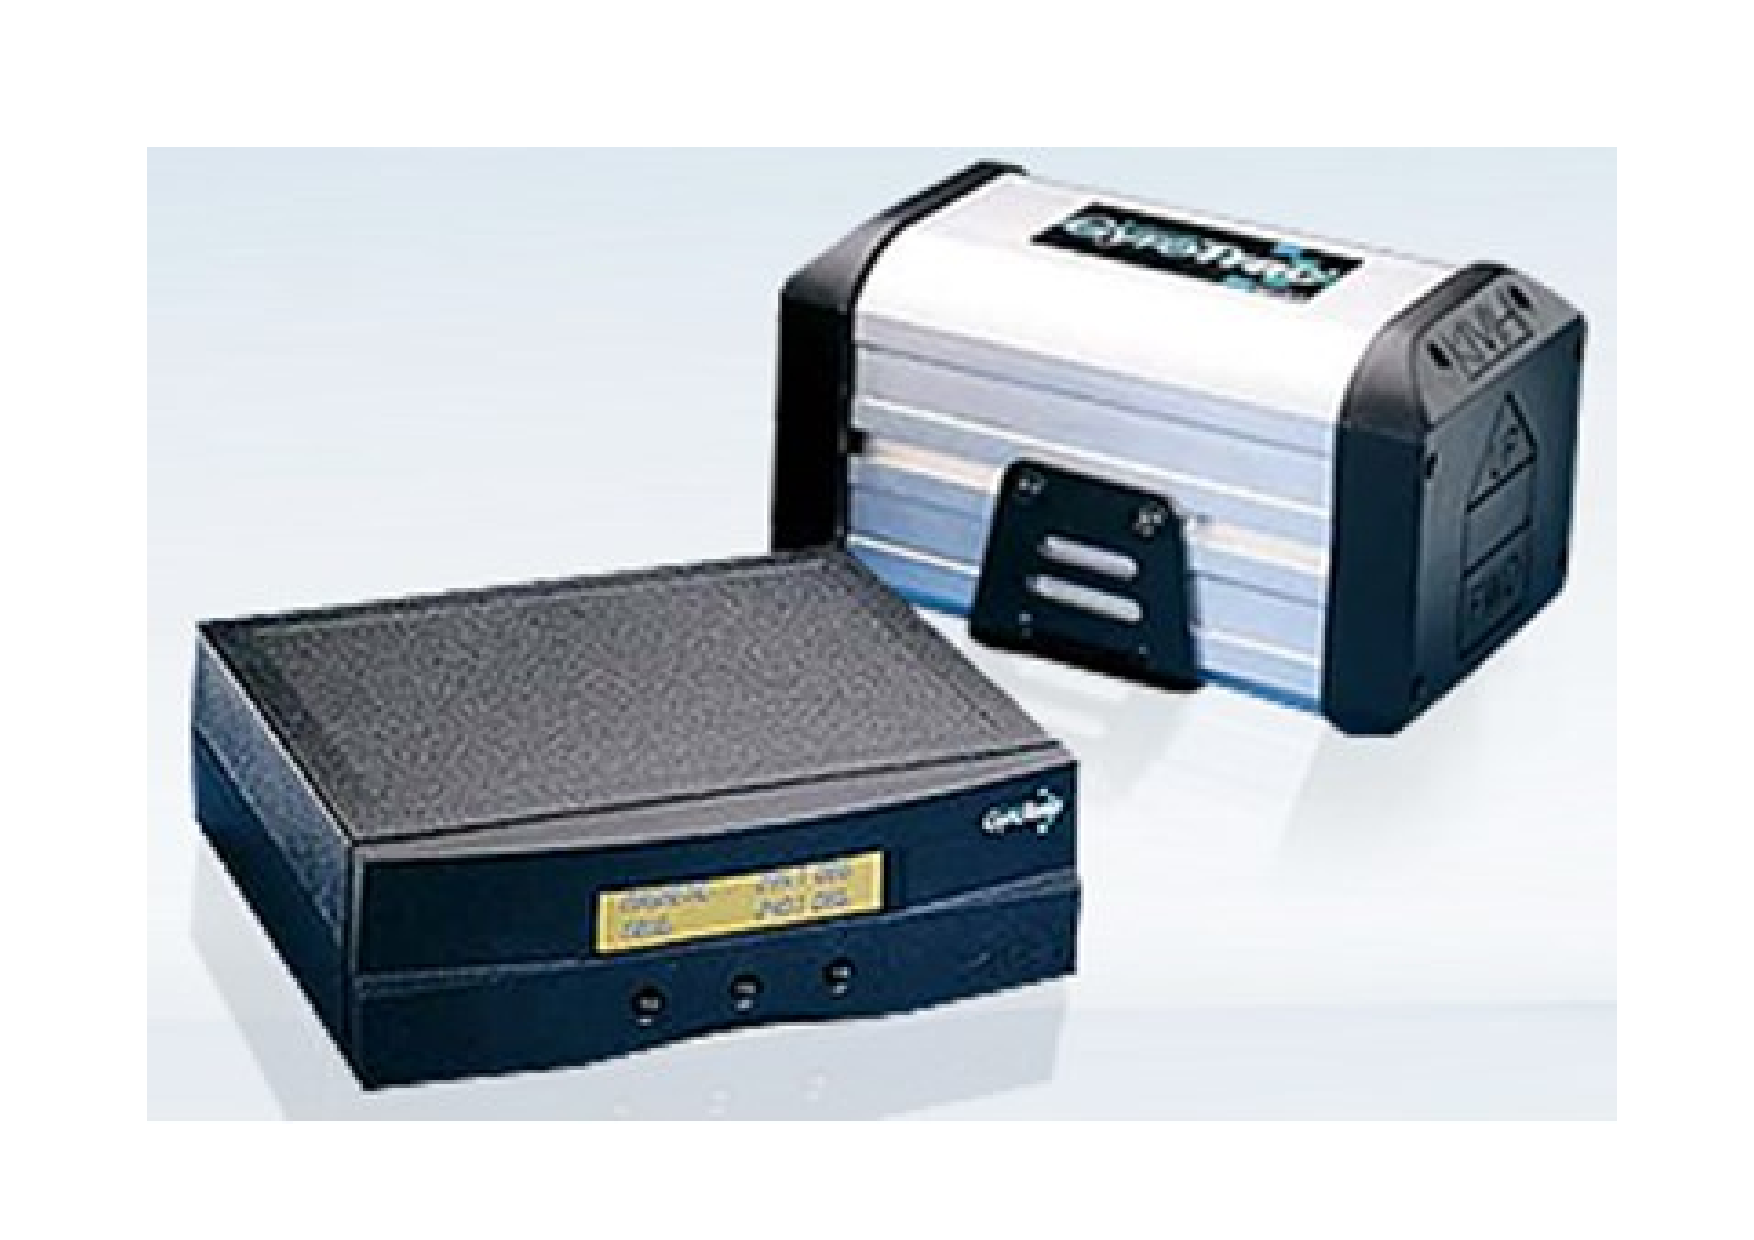
\includegraphics[height=4cm]{Vaje/VzorecPoroc/figs/Gyrotrac_slika.pdf}
	%
	% If not, use
	%\picplace{5cm}{2cm} % Give the correct figure height and width in cm
	%
	\caption{Uporabljeni kompas Gyrotrack s prikazovalnikom ADCU}
	\label{fig:GT}       % Give a unique label
\end{figure}

\subsubsection{Vrtavčni ali žiro kompas}
Giro kompas ali žiro kompas je kompas, ki kaže prave smeri v naravi. Njegov osnovni del je žiroskop, dinamični in simetrično telo, ki se vrti okoli svoje osi s hitrostjo 20000 obratov na minuto ali več. Osnovna lastnost žiroskopa je ta, da se os rotacije postavi pravokotno na silo, ki na njo vpliva. Napake, ki so za navigacijo zanemarljive, nastanejo zaradi:
\begin{itemize}
	\item \textbf{Coriolisove sile}: zaradi nje se os rotacije postavi v smeri sever - jug
	\item \textbf{gravitacije}: zaradi nje se os rotacije nagiba proti ravnini horizonta
	\item \textbf{hitrosti} gibanja oz. zavijanja ladje in
	\item \textbf{smeri} plovbe: v smereh $090^{\circ}$ in $270^{\circ}$ vrtavčni kompas nima napake
\end{itemize}


\subsection{Delo s kompasom Gyrotrac}
%\label{sec:2}
Kompas GyroTrac je žiroskopsko stabilizirani digitalni magnetni kompas brez gibljivih delov. Torej na njega, prav tako kot na magnetni kompas, vpliva magnetno polje Zemlje, feromagnetni objekti v okolju na katere vpliva magnetno polje in trajni magneti v okolici. Torej ima GyroTrac napake zaradi variacije in deviacije, vendar so le-te zmanjšane s pomočjo triosnih giroskopov.

\begin{figure}
	\centering
	% Use the relevant command for your figure-insertion program
	% to insert the figure file.
	% For example, with the option graphics use
	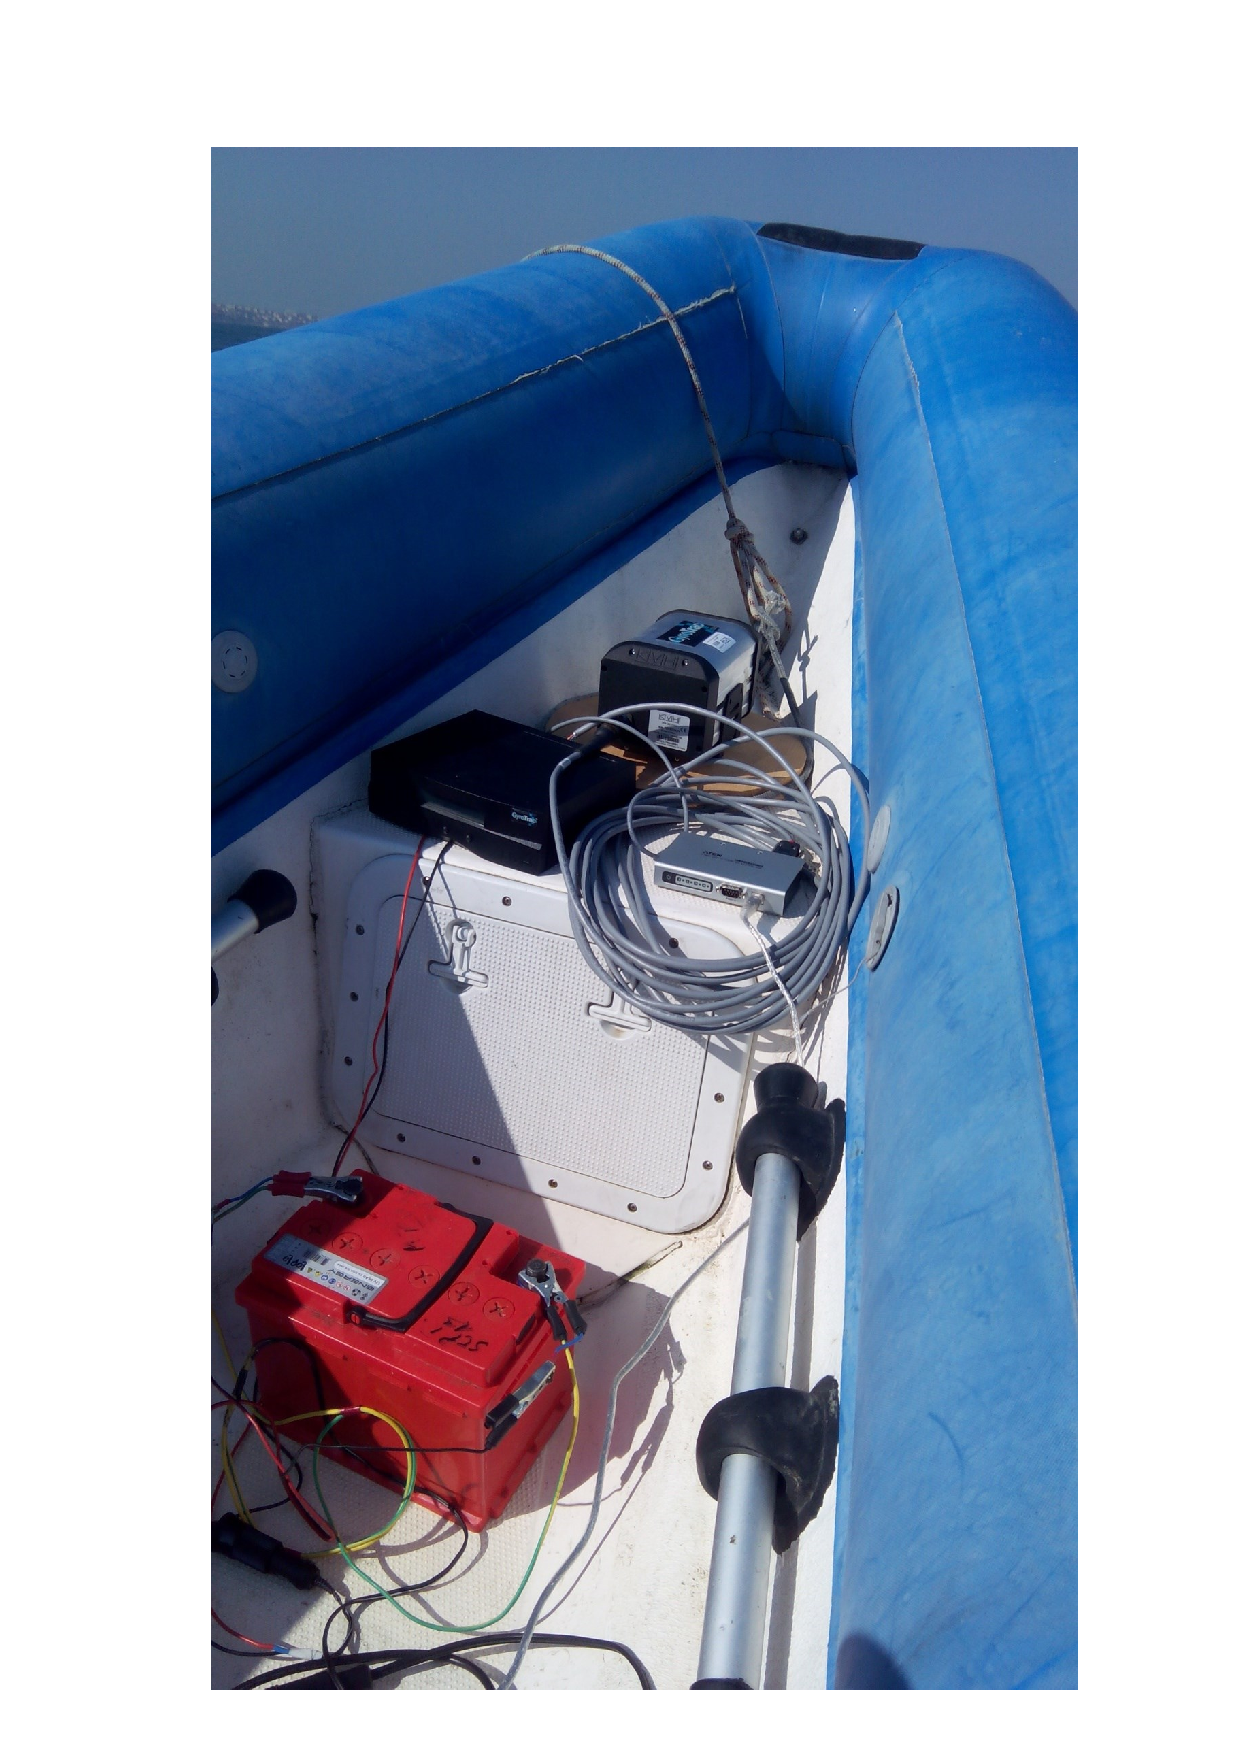
\includegraphics[height=8cm]{Vaje/VzorecPoroc/figs/Postavitev_gumenjak.pdf}
	%
	% If not, use
	%\picplace{5cm}{2cm} % Give the correct figure height and width in cm
	%
	\caption{Postavitev girokompasa in ostalih naprav na gomonu}
	\label{fig:GT_gum}       % Give a unique label
\end{figure}

\begin{figure}
	\centering
	% Use the relevant command for your figure-insertion program
	% to insert the figure file.
	% For example, with the option graphics use
	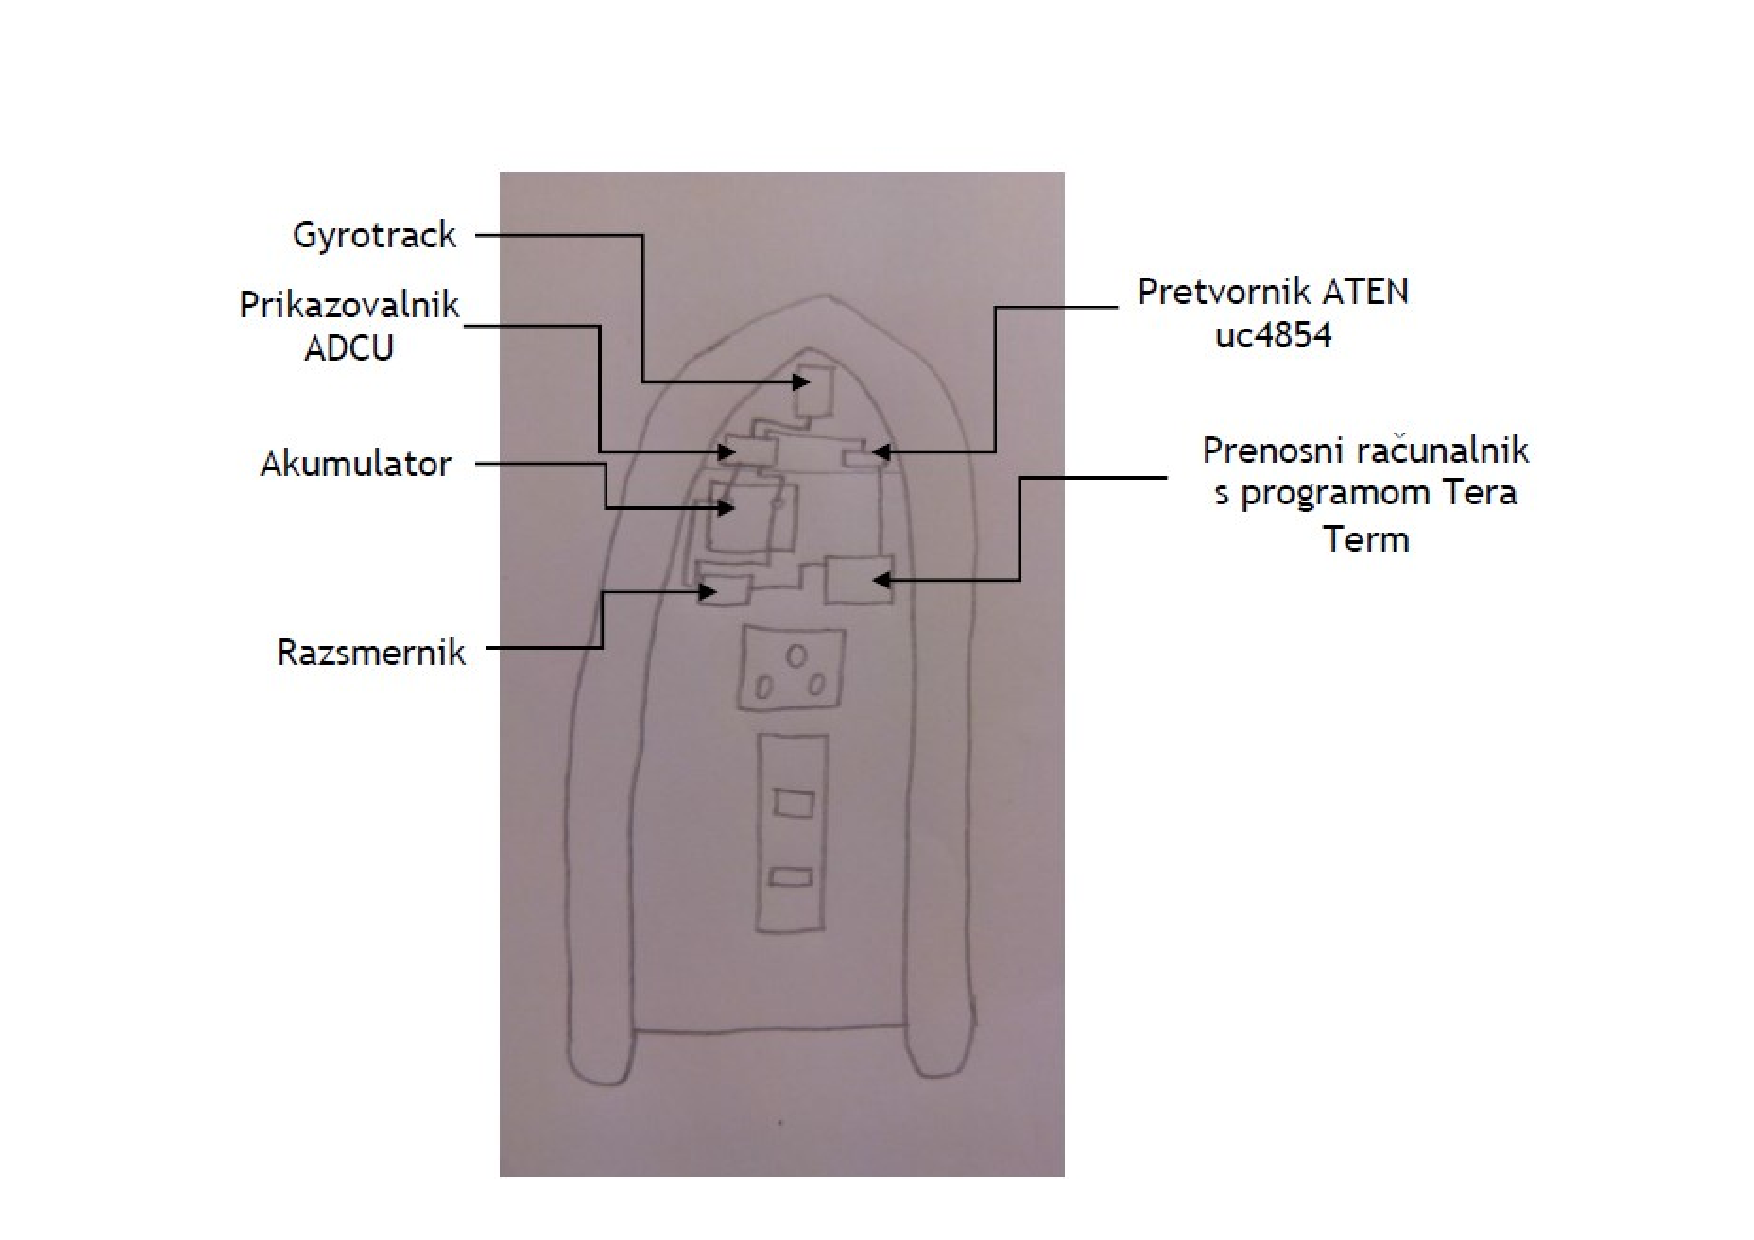
\includegraphics[height=9cm]{Vaje/VzorecPoroc/figs/Razporeditev_opreme.pdf}
	%
	% If not, use
	%\picplace{5cm}{2cm} % Give the correct figure height and width in cm
	%
	\caption{Skica postavitve naprav na gomonu}
	\label{fig:gum_tloris}       % Give a unique label
\end{figure}


\subsubsection{Statična napaka na terenu}
Najprej smo opravili meritve na morju in sicer, azimut pokrite smeri na svetilnika na vhodu v mandrač Bernardin (R.Bl.3s6m3M in Z.Bl.3s6m3M) je znašal $5,5^{\circ}$, azimut izmerjen na karti pa $10,0^{\circ}$ (skica karte). Torej iz tega sledi da je napaka girokompasa $4,5^{\circ}$. Po formuli znaša deviacija girokompasa: $\delta_g = \omega_p - \omega_g$. Pri čemer je $\omega_p = 10,0^{\circ}$ in $\omega_g = 5,5^{\circ}$.
Girotrack bi sicer moral kazati smer s točnostjo $\pm 1^{\circ}$, vendar je do take napake lahko prišlo zaradi vpliva magnetnega polja v okolici, torej variacije, ki je v območju merjenja trenutno znašala $2^{\circ}45'E$ ter zaradi slabega morja in vetra, zaradi katerih je bilo gomon težje obdržati v smeri.

\begin{figure}
	\centering
	% Use the relevant command for your figure-insertion program
	% to insert the figure file.
	% For example, with the option graphics use
	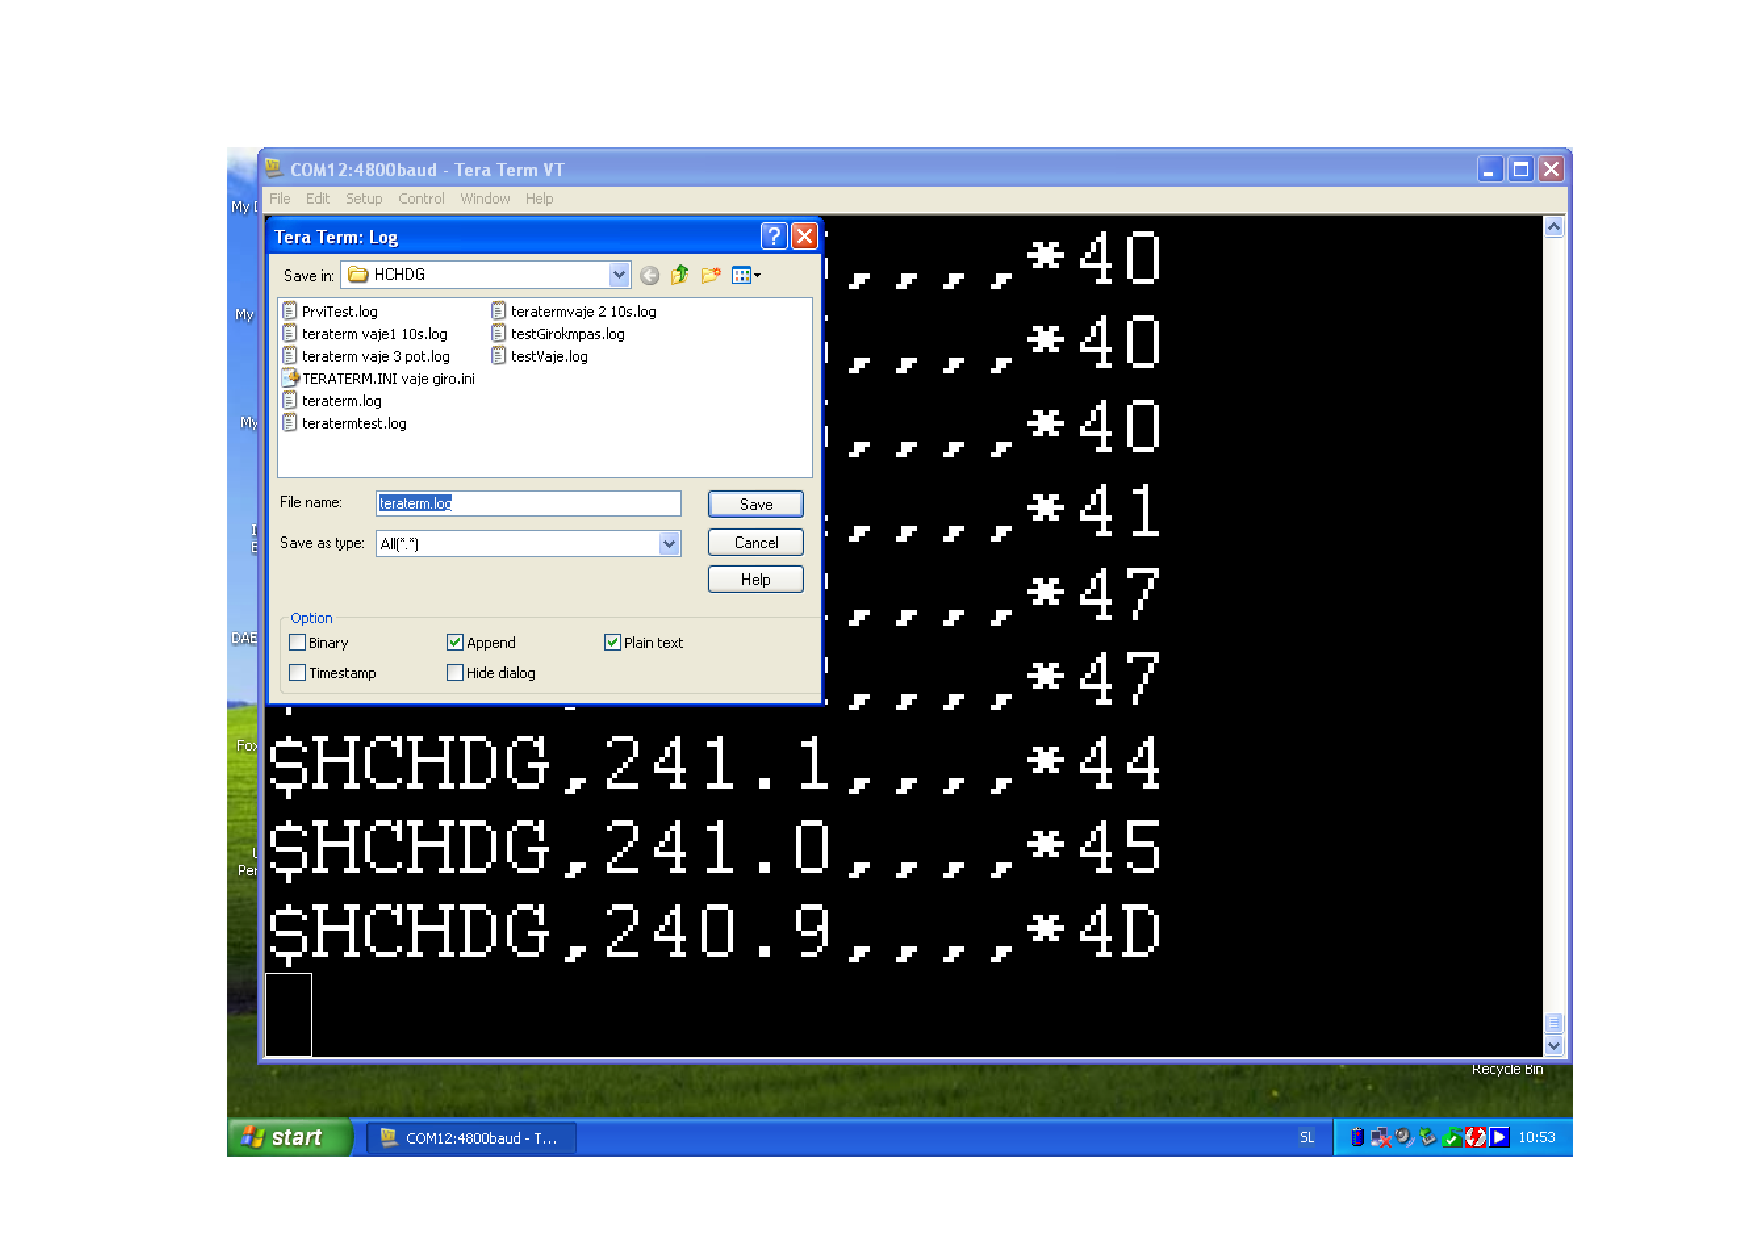
\includegraphics[height=6cm]{Vaje/VzorecPoroc/figs/IzbiraDatoteke.pdf}
	%
	% If not, use
	%\picplace{5cm}{2cm} % Give the correct figure height and width in cm
	%
	\caption{Izbira datoteke kamor nam program Tera Term zapisuje in shrani podatke}
	\label{fig:TT_datotek}       % Give a unique label
\end{figure}

\begin{figure}
	\centering
	% Use the relevant command for your figure-insertion program
	% to insert the figure file.
	% For example, with the option graphics use
	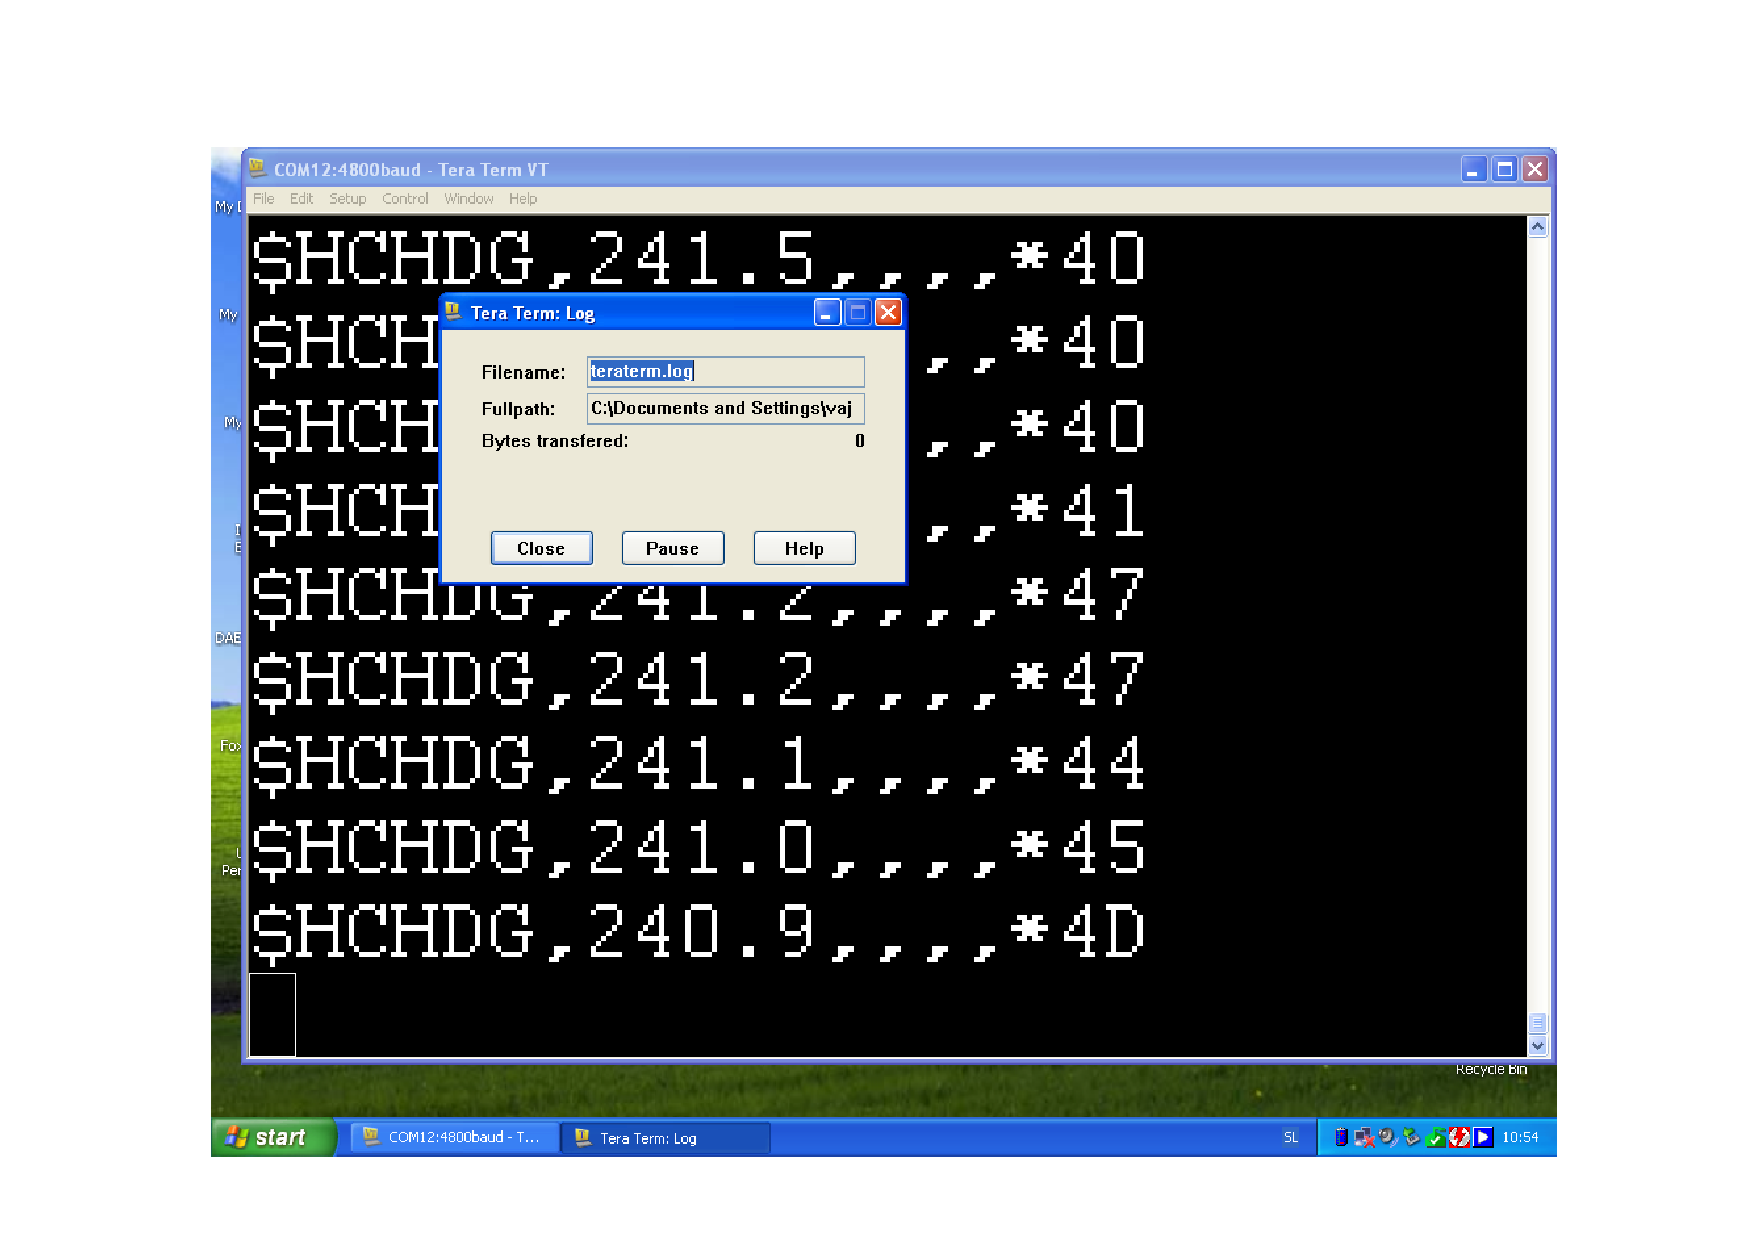
\includegraphics[height=6cm]{Vaje/VzorecPoroc/figs/ShranDatoteke.pdf}
	%
	% If not, use
	%\picplace{5cm}{2cm} % Give the correct figure height and width in cm
	%
	\caption{Okno, ki se odpre, ko program začne shranjevati podatke}
	\label{fig:TT_shran}       % Give a unique label
\end{figure}

\subsubsection{Dinamična napaka na morju}
Nato smo na morju merili še reakcijski oz. stabilizacijski čas girokompasa. To smo izvedli tako, da smo pri vožnji s 3 vozli opravili obrat za $105^{\circ}$ in sicer iz smeri $200^{\circ}$ smo obrnili v smer $095^{\circ}$ ter merili čas, so se se prikazovalni podatki girokompasa umirli. Ta čas je znašal pet sekund.
\begin{figure}
	\centering
	% Use the relevant command for your figure-insertion program
	% to insert the figure file.
	% For example, with the option graphics use
	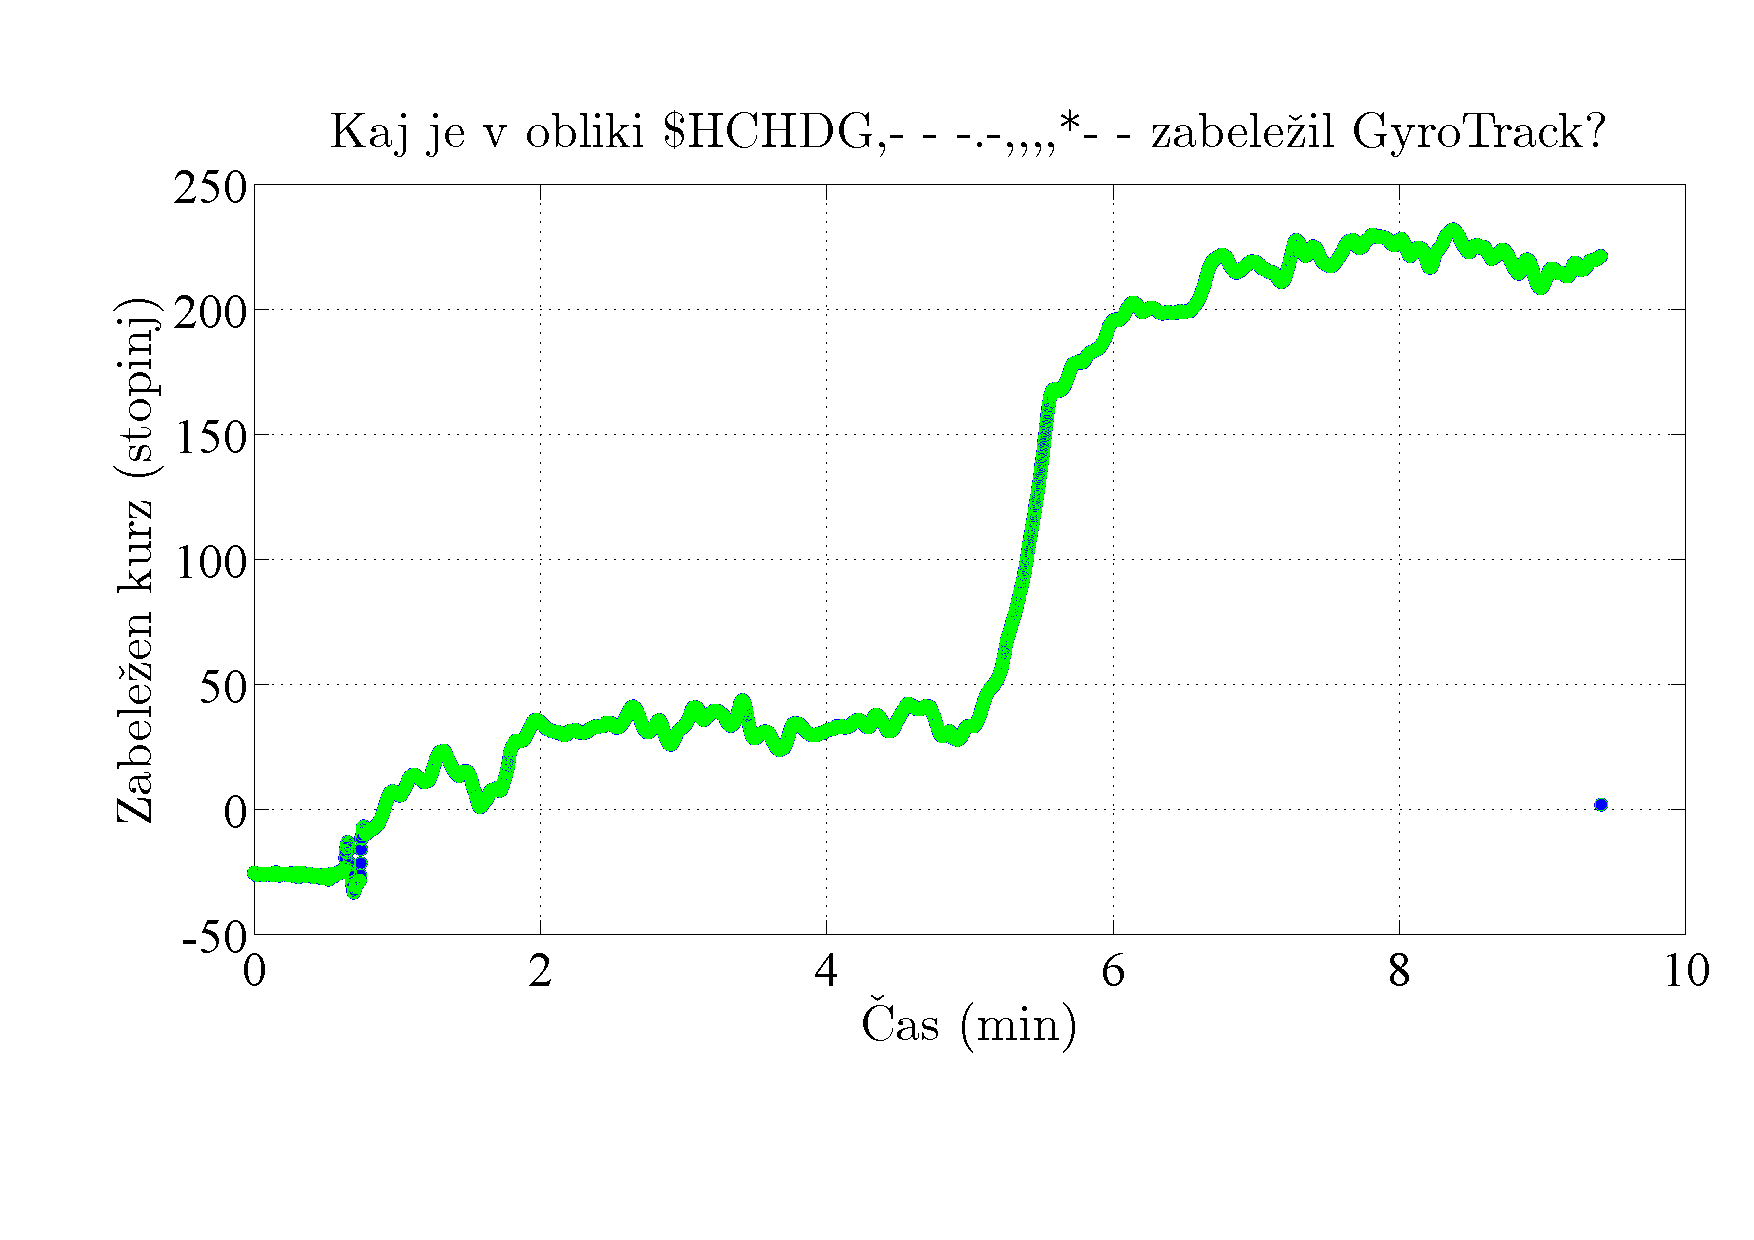
\includegraphics[height=6cm]{Vaje/VzorecPoroc/figs/2014-04-10_KurzPoti_Gyrotrack.pdf}
	%
	% If not, use
	%\picplace{5cm}{2cm} % Give the correct figure height and width in cm
	%
	\caption{Graf zapisovanja kurza med plovbo, zabeleženo na sliki \ref{fig:GyroGps_sled}}
	\label{fig:Gyro_krog}       % Give a unique label
\end{figure}


\subsubsection{Krog na morju}
Opravili smo še en poizkus na morju. Vse naprave smo povezali z računalnikom ter s programom Tera Term. V tem programu smo izbrali funkcijo Log in program je začel shranjevati podatke girokompasa.

\begin{figure}
	\centering
	% Use the relevant command for your figure-insertion program
	% to insert the figure file.
	% For example, with the option graphics use
	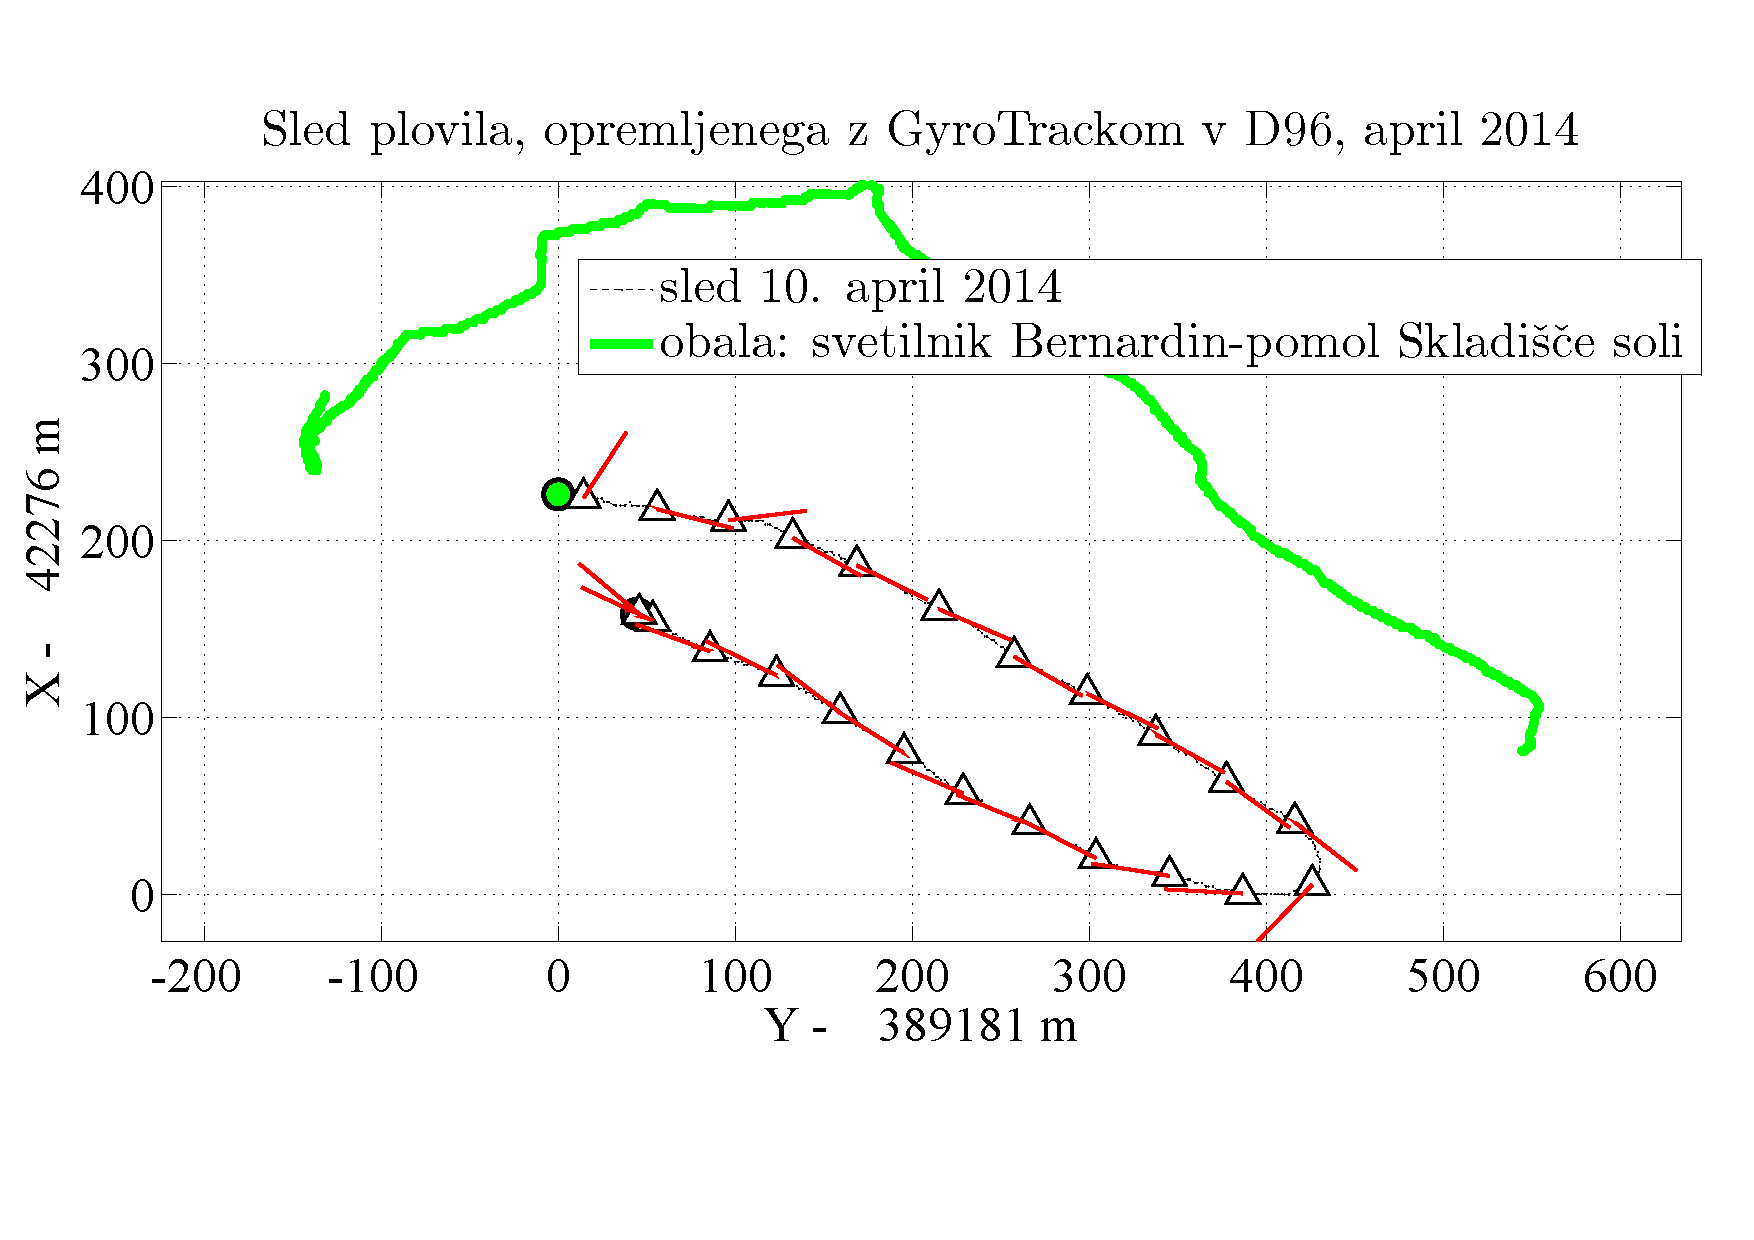
\includegraphics[height=6cm]{Vaje/VzorecPoroc/figs/SledPlovilaZGyrotrackom_KurzSamoOdNmeaGps.pdf}
	%
	% If not, use
	%\picplace{5cm}{2cm} % Give the correct figure height and width in cm
	%
	\caption{Vris kombinirane sledi plovila iz GPS in kurza iz Gyrotrac-a (meritev s slike \ref{fig:Gyro_krog} ) poleg obalne črte, dobljene z GPS.}
	\label{fig:GyroGps_sled}       % Give a unique label
\end{figure}

Usposobili smo tudi še GPS, ki si je sproti zapisoval podatke. Izvedli smo zajem podatkov med plovbo, ki je trajala točno 7,0 minut. Podatke, ki jih je program Tera Term shranil v računalnik, smo odprli s programom Excel, jih prešteli in ugotovili, da Gyrotrac zapisuje 8 podatkov na sekundo. To smo izračunali tako, da smo število podatkov delili s časom trajanja vožnje. Torej merili smo 7 minut, kar je enako 420 sekund, v tem času se je nabralo 3353 vrstic podatkov.

$$ 3353\,vrstic : 420\,s = 7,98\,vrstic/s \equiv 8\,vrstic/s $$


\subsubsection{Statična napaka, izmerjena na kopnem}
Ko so bile meritve na morju opravljene, smo opravili še meritve na obali.  Gyrotrac smo postavili na trinožno stojalo in izmerili pokrito smer svetilkov na Bernardinu, in sicer svetilnika R.Bl.3s6m3M in R.Bl.5s9m3M, ki je znašala $239,5^{\circ}$. To vrednost smo primerjali z vrednostjo izmerjeno na karti, ki je bila $240,6^{\circ}$ in ugotovili, da je napaka girokompasa tokrat znašala $1,1^{\circ}$. 

\begin{figure}
	\centering
	% Use the relevant command for your figure-insertion program
	% to insert the figure file.
	% For example, with the option graphics use
	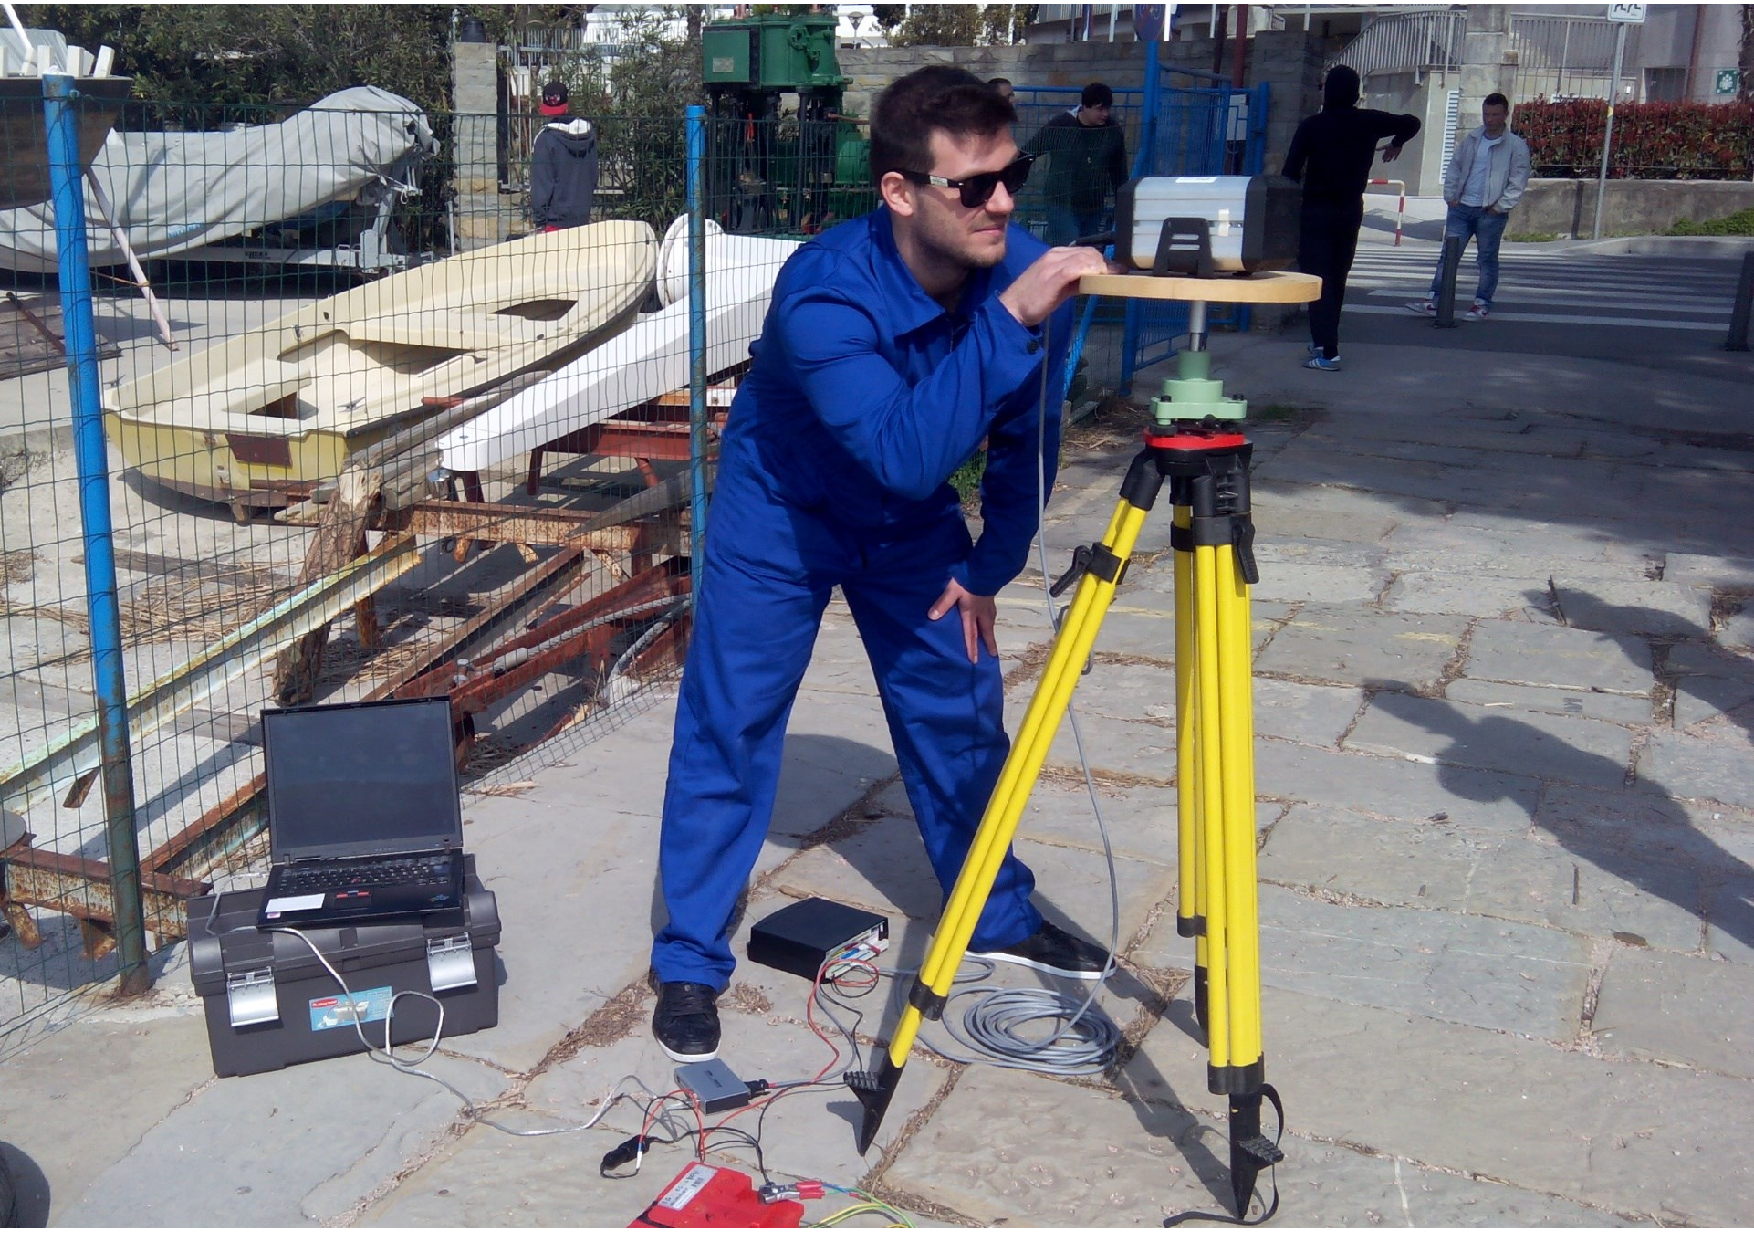
\includegraphics[height=5cm]{Vaje/VzorecPoroc/figs/Aleks_Gyro.pdf}
	%
	% If not, use
	%\picplace{5cm}{2cm} % Give the correct figure height and width in cm
	%
	\caption{Merjenje azimuta z girokompasom na stojalu}
	\label{fig:Aleks_meri}       % Give a unique label
\end{figure}


Iz tega lahko sklepamo, da napaka variacije ne vpliva znatno na Gyrotrack kompas in je bila napaka izmerjena na morju vpliv močnega vetra ter nezmožnosti obdržati gomon dovolj dobro v smeri, da bi lahko izmerili dovolj natančen azimut. Izmerili smo še azimut na svetilik pred vhodom v Portoroško marino (Z.Bl.4s8m4M), ki je bil $139,0^{\circ}$.

\begin{figure}
	\centering
	% Use the relevant command for your figure-insertion program
	% to insert the figure file.
	% For example, with the option graphics use
	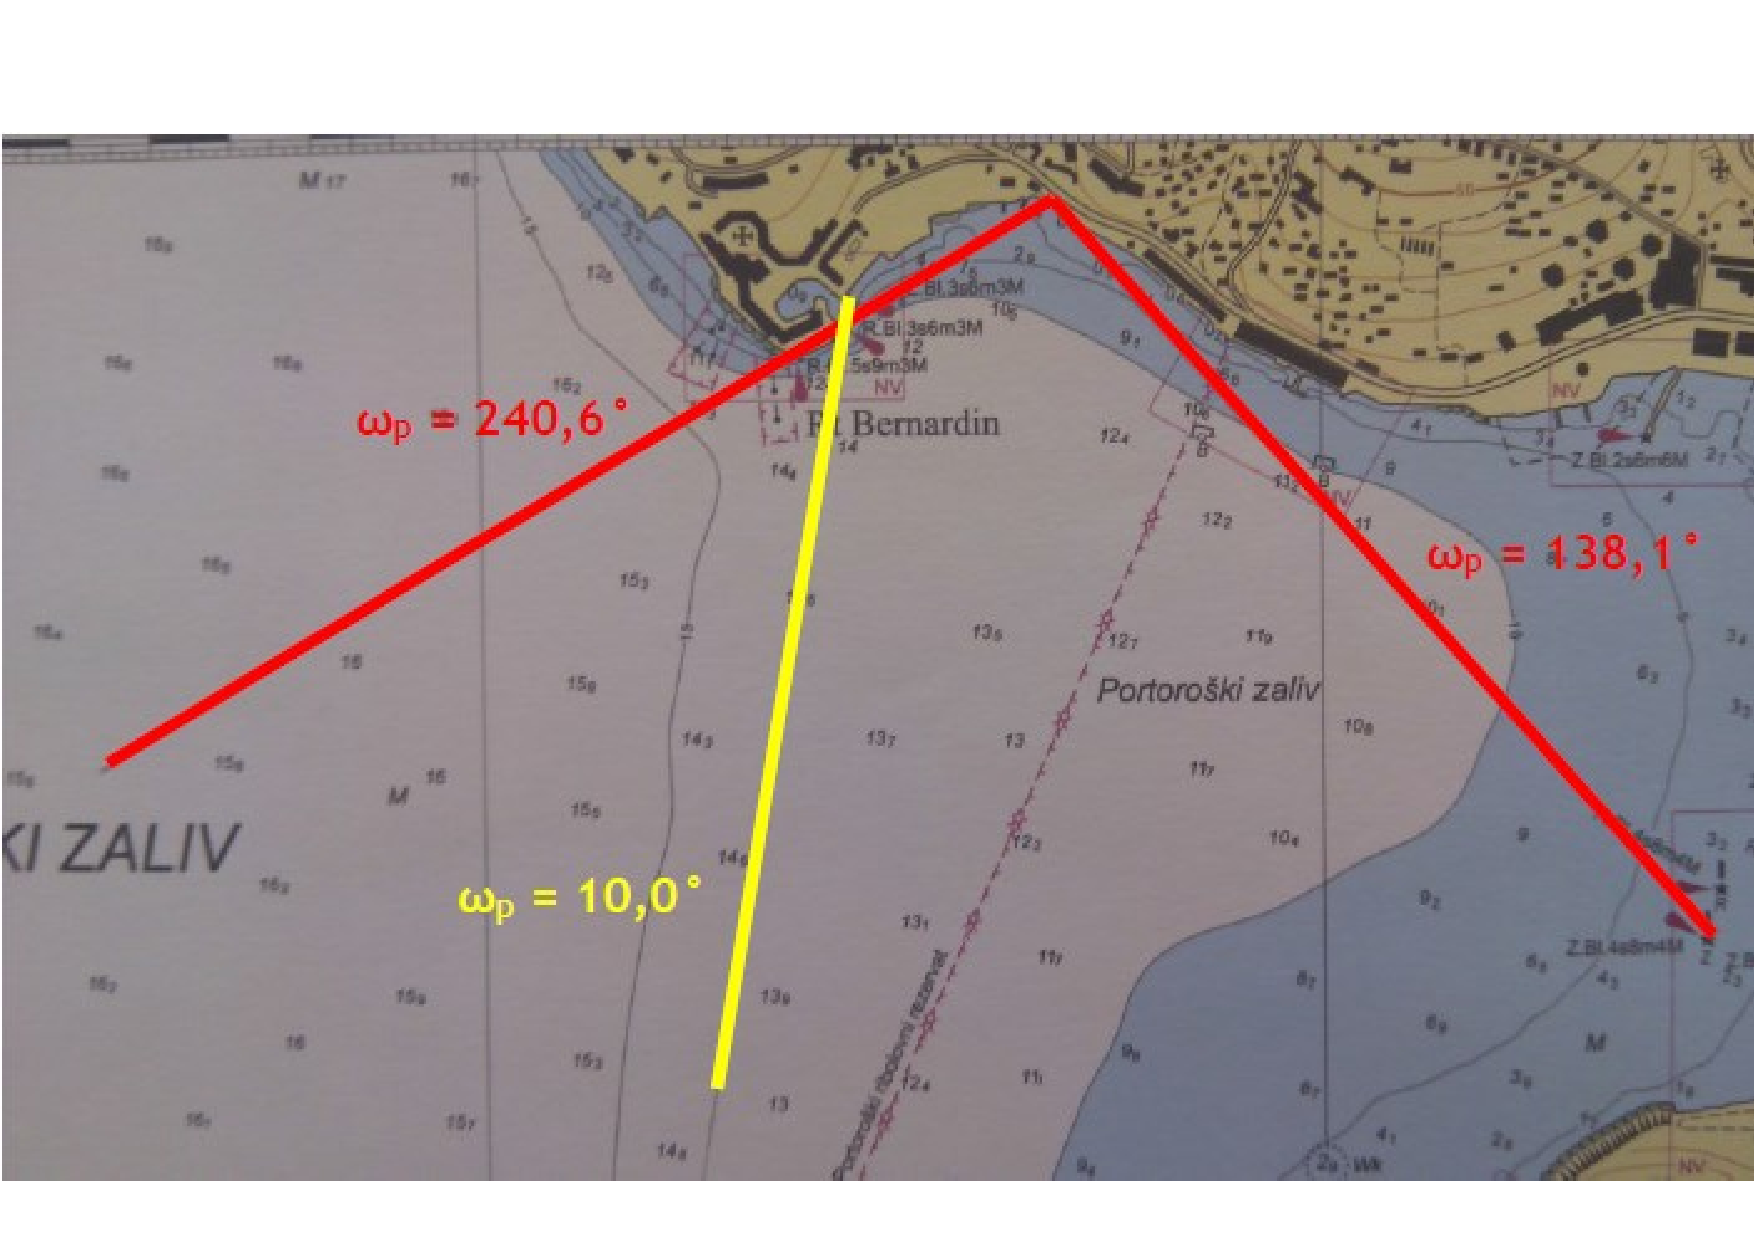
\includegraphics[height=5cm]{Vaje/VzorecPoroc/figs/Karta_Azimuti.pdf}
	%
	% If not, use
	%\picplace{5cm}{2cm} % Give the correct figure height and width in cm
	%
	\caption{Izmerjeni azimuti (rdeči - meritve z obale, rumeni - meritve z morja)}
	\label{fig:Karta_IzmerAzimuti}       % Give a unique label
\end{figure}



\begin{figure}
	\centering
	% Use the relevant command for your figure-insertion program
	% to insert the figure file.
	% For example, with the option graphics use
	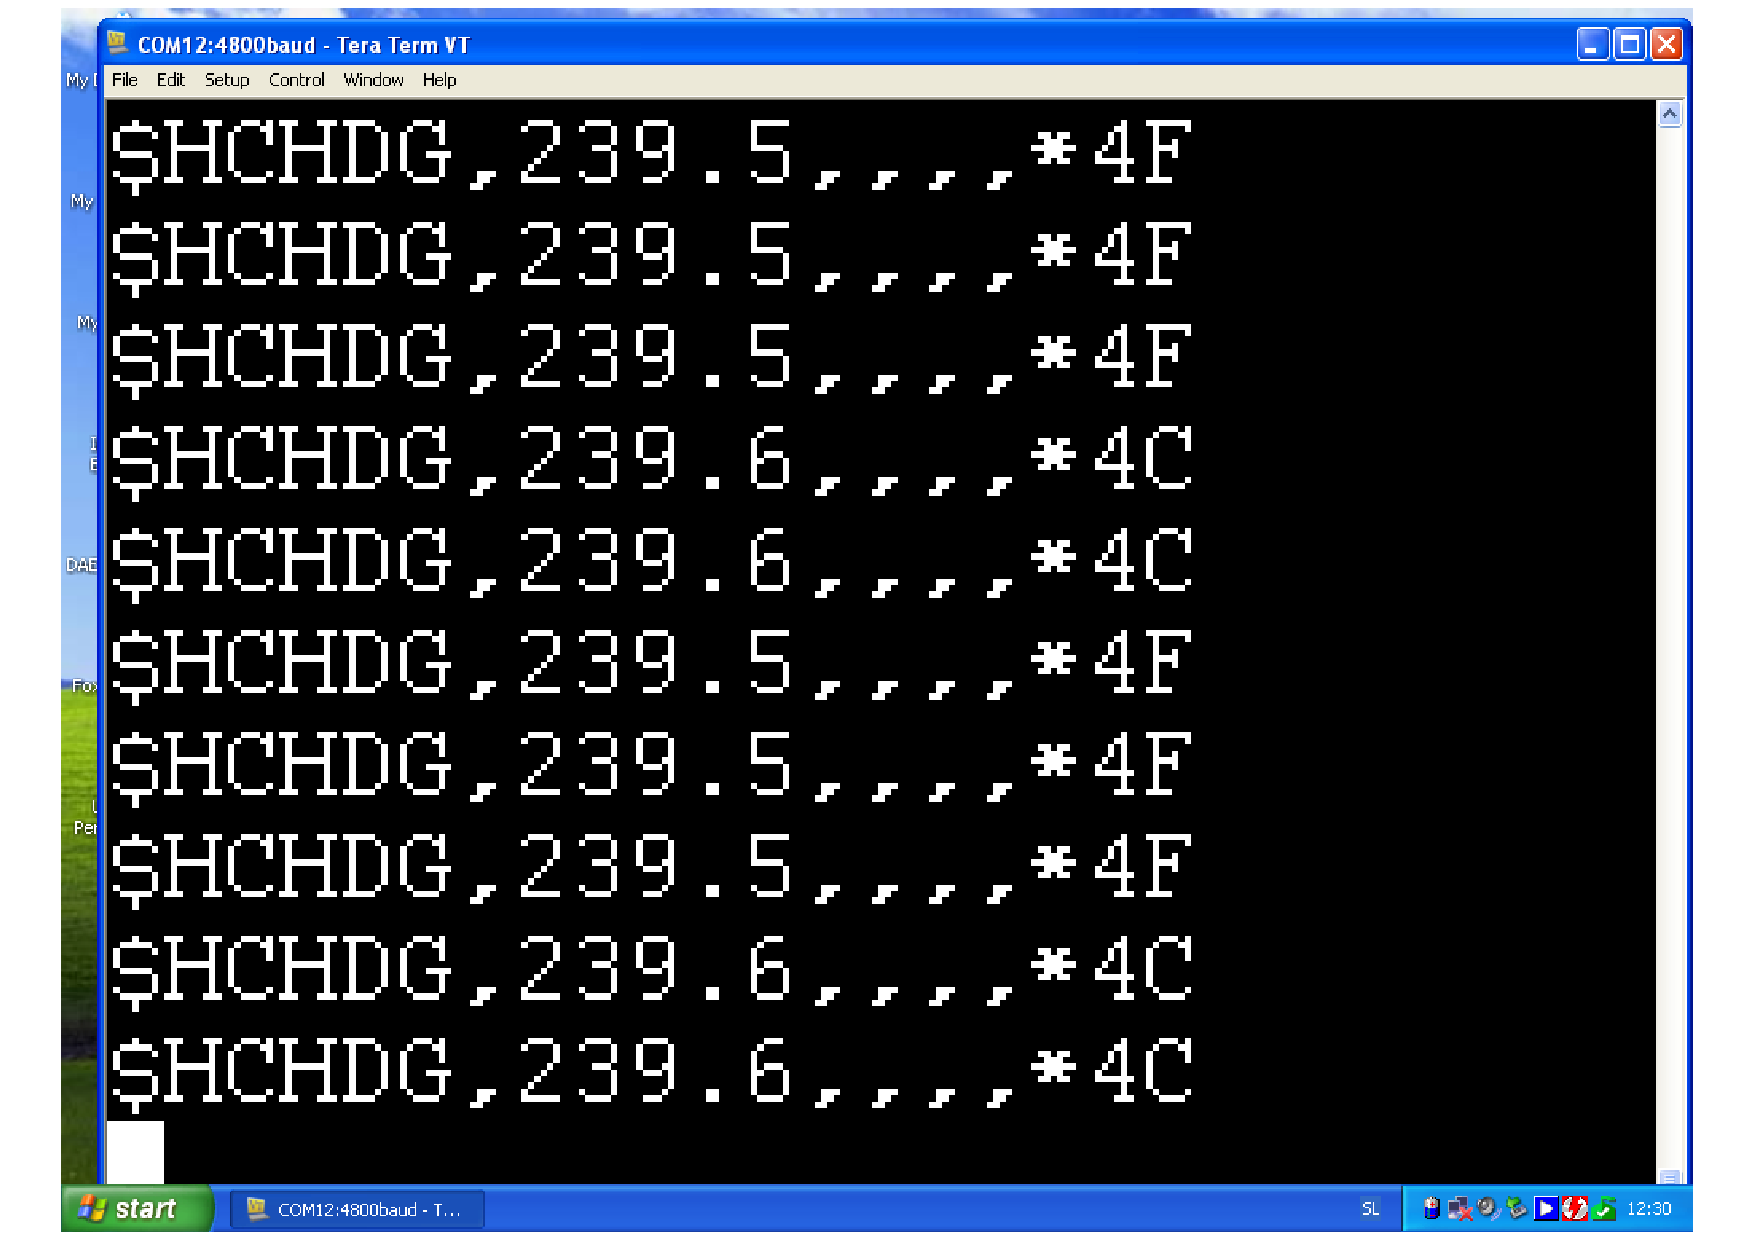
\includegraphics[height=4cm]{Vaje/VzorecPoroc/figs/TT_zapisovanje.pdf}
	%
	% If not, use
	%\picplace{5cm}{2cm} % Give the correct figure height and width in cm
	%
	\caption{Zapisovanje izmerjenih podatkov v pokriti smeri s programom Tera Term}
	\label{fig:TT_zapisovanjePokriteSmeri}       % Give a unique label
\end{figure}

Gyrotrac je bil postavljen na kamnitem pomolu pred vhodom v čolnarno. Azimut smo izmerili še na karti in $138,1^{\circ}$. Iz tega sledi, da je bila tokrat \textbf{napaka kompasa} $0,9^{\circ}$. Ovrgli smo nezanesljiv rezultat, ki smo ga dobili med meritvijo na morju v močnem vetru. 

\textbf{Reakcijskega časa} Gyrotraca nismo izmerili, zanesemo se na rezultate \ref{fig:StabRez}, ki so lani z laboratorijskimi meritvami izmerili naši predhodniki \cite{Girokompas_2013}. Po naši oceni rabi odčitek smeri Gyrotraca približno 10 sekund, da se po zelo sunkovitem zasuku zadovoljivo ustali v novi smeri.

\begin{figure}
	\centering
	% Use the relevant command for your figure-insertion program
	% to insert the figure file.
	% For example, with the option graphics use
	%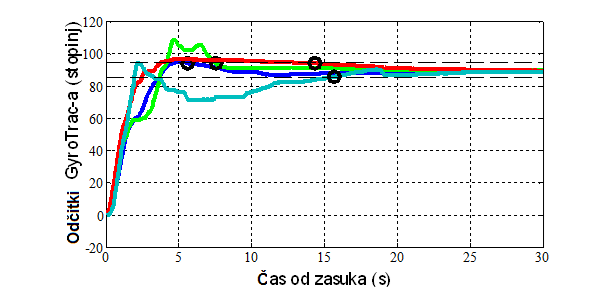
\includegraphics[height=5cm]{Vaje/VzorecPoroc/figs/Gyro_casOdziva.png}
	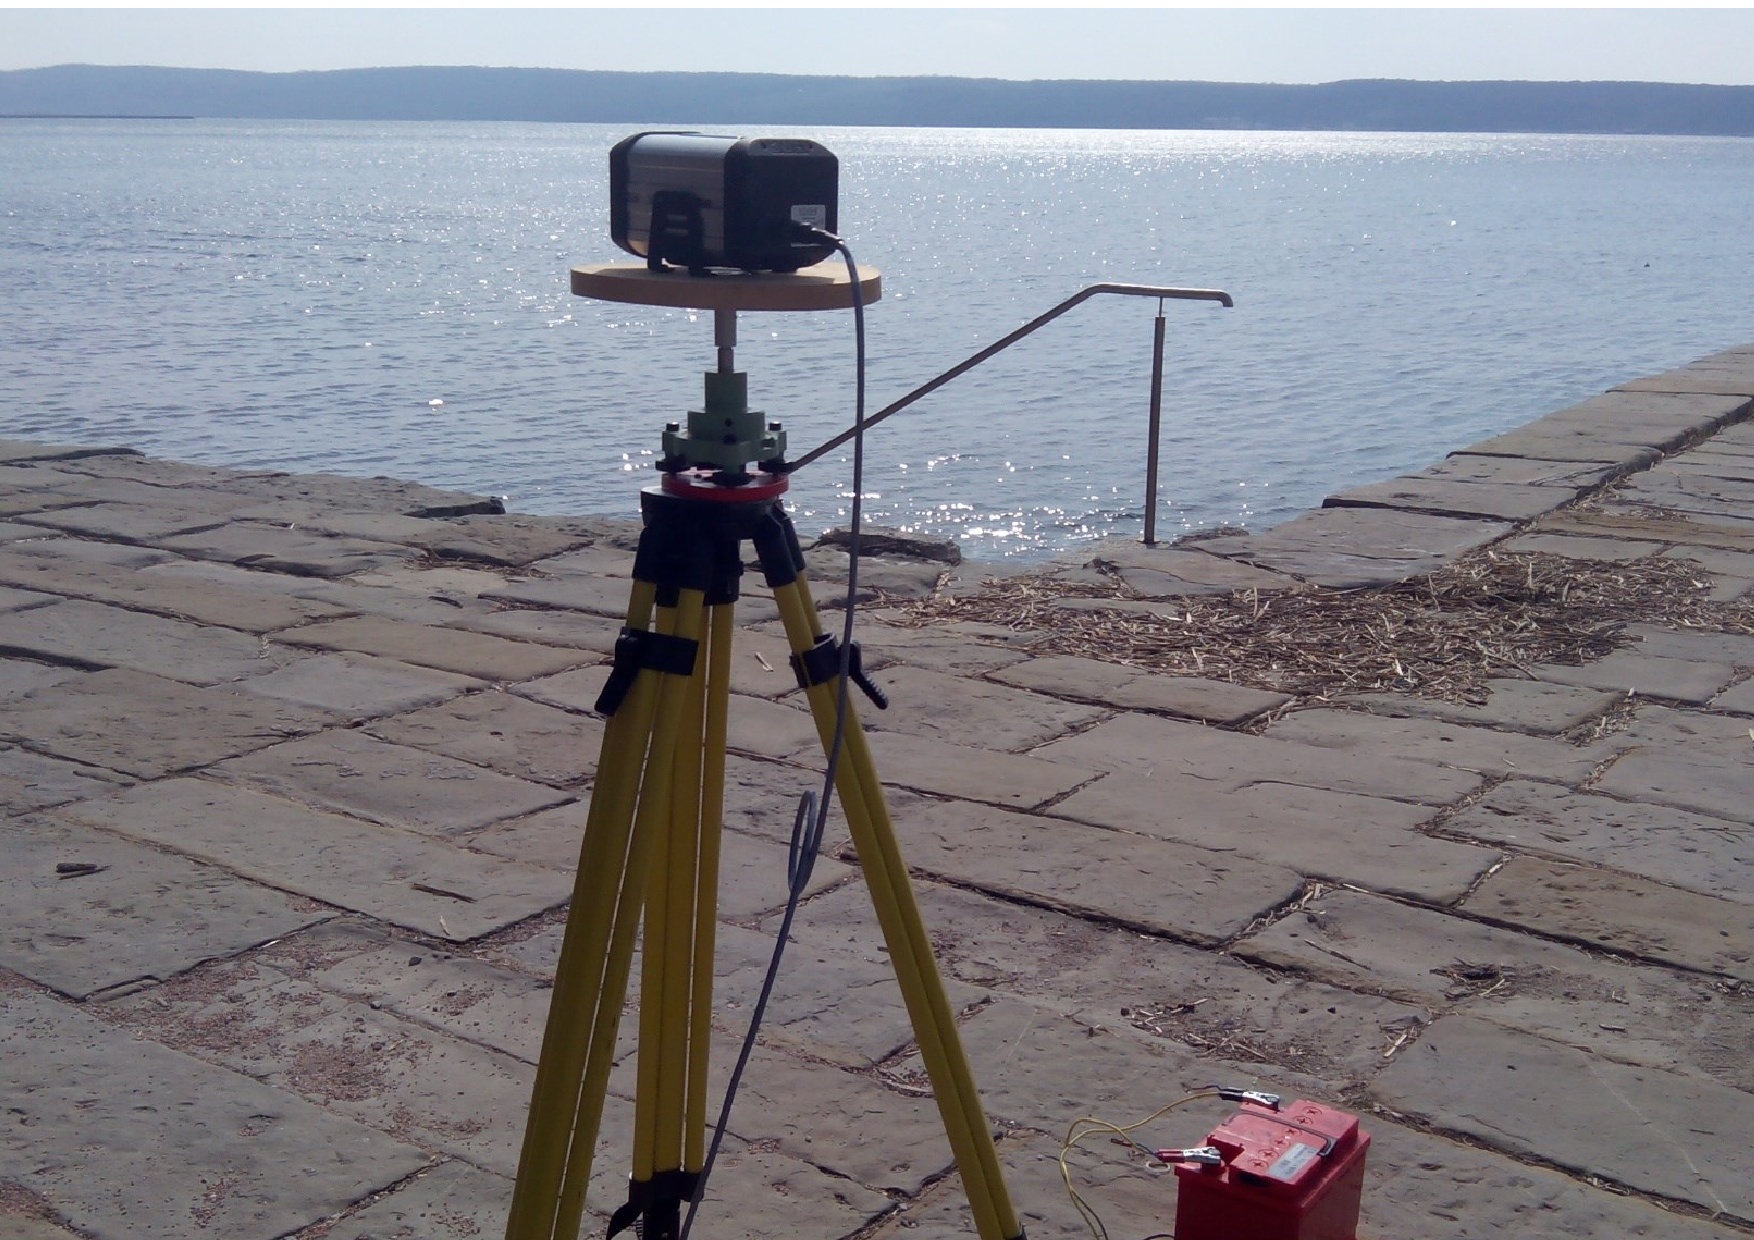
\includegraphics[height=5cm]{Vaje/VzorecPoroc/figs/Gyro_obala}
	%
	% If not, use
	%\picplace{5cm}{2cm} % Give the correct figure height and width in cm
	%
	\caption{Stabilizacija podatkov GyroTrac v območje $\pm5^{\circ}$, ko so senzorski del sunkovito zasukali za $90^{\circ}$  \cite{Girokompas_2013}}
	\label{fig:StabRez}       % Give a unique label
\end{figure} 


\subsection{Koristi za naše bodoče delo}
\label{sec:2}
V pomorstvu je napaka kompasa lahko usodna,  ko nam ostale naprave odpovejo. Zato se na ladji vodi napako kompasa v vsaki straži s pomočjo svetilnikov, zvezd, objektov. To je bila zelo koristna vaja, saj na tak praktičen način spoznavamo naše delo in v bistvu vidimo, kaj je sploh ta napaka, katero upoštevamo ob vrisovanju položajev in vrisovanju azimutov pri pouku obalne navigacije. Znati popravit to napako je osnova navtike. Seveda pa smo tudi uživali v vožnji s čolnom se naučili pristati in privezati ladjo, pri čemer je prišel do izraza \textit{team building}. Upamo, da smo vam jasno predstavili in povedali koliko je v resnici pomembno znanje popravka kompasa.

\subsection{Pisanje poročila}
\label{ch:seminar_report_template}
Poročilo je potrebno napisati v \LaTeX $\:$  okolju. Predloga poročila se nahaja na linku: \href{https://github.com/UNI-LJ-FPP/LEN/tree/master/seminar/naloge/template_naloga_XX}{github.com/UNI-LJ-FPP}, kjer je tudi navodilo. 


%\bibliographystyle{plain}
%\bibliography{literatura}

%
